Unlike elliptic curves, when the genus of a curve is greater than one, then the set of points on it will not always form a group. 

\subsection{The Jacobian of a Hyperelliptic Curve}

Luckily, there is another way to form an abelian group with hyperelliptic curves. Indeed, let $D$ be the set of all formal finite sums 

$$ \sum_i m_i P_i $$ 

where $m_i \in \mathbb{F}_p$ and $P_i$ are points on the curve $H$. We call elements of $D$ divisors of $H$. Given a rational function $f$ in $\mathbb{F}_p(H)$, we can define the corresponding divisor to $f$ as

$$(f) = \sum_i m_i P_i $$ where $P_i$ are the zeros and poles of $f$ with number of multiplicities $m_i$. Divisors of this form are called principal divisors and we let $P$ denote the subset of all of them in $D$. If we define the operation on $D$ by 

$$ \sum_i m_i P_i  + \sum_i m^\prime_i P_i  = \sum_i (m_i+m^\prime) P_i $$ 

then $D$ becomes and abelian group. Unfortunetly, this group is far too large and unstructured for cryptographic purposes. So we consider the subgroup $D^0$ of all divisors of $D$ whose coefficients sum to $0$. That is, divisors $ \sum_i m_i P_i $ such that $\sum_i m_i = 0$. This subgroup is still infinite, but that can be remedied by defining two divisors $D_1, D_2$ of $D^0$ to be equal if $D_1 - D_2$ is equal to the divisor of a rational function on $H$. That is, $D_1 - D_2 = (f) $ for $f \in \mathbb{F}_p(H)$. This new quotient group, denoted $$J = D^0 / P$$ is called the jacobian of the curve $H$ and is a finite cyclic group. Since elements of $J$ are in fact equivalence classes of divisors we use the symbol $[D]$ to represent them. This will be the group used to build hyperelliptic cryptosystems.

\subsection{Representation of Divisors}

Athough the Jacobian $J$ of an hyperelliptic curve $H$ is a finite abelian group, elements of $J$ can be very hard to represent. To make the group operation in $J$ reasonable, we ustilize the Mumford representation of a divisor which is described as follows. We call a divisor $D$ \textit{semi-reduced} if 
$$D = \sum_{P\in H \backslash \OV} m_PP - \sum_{P\in H \backslash \OV}m_P\OV$$ satisfies  
\begin{enumerate}[(i)]
	\item $m_i \geq 0$
	\item If $P \neq P^{\prime}$ and $m_P> 0$, then $m_{P^\prime} = 0$
	\item If $P=P^\prime $ and $m_P> 0$, then $m_p = 0$
\end{enumerate} 
A semi-reduced divisor $D$ is completely reduced if $D= \sum_{P\in H}m_P \leq \mathfrak{g}$. It turns out that for every equivalence class $[D]$ in $J$ there exists an unique reduced divisor $D^\prime$ such that $[D\prime] = [D]$. An interesting consequence is that every element in $J$ can be represented with the sum of $\mathfrak{}g$ points. So for a hyperelliptic curves of genus $2$, there are elements of $J$ which cannot be represented with less than $2$ points. In the case of elliptic curves, the genus is $1$, so $J \cong E$.  This also means that acurately storing all reduced divisors is equivalent to storing all of $J$ on a computer! Although this is convenient, the presentation is still combersome. Ideally, we would like to represent divisors algebraically, which is what the Mumford representation allows us to do. Let $D$ be a semi-reduced with points $P_i = (x_i,y_i)$. We associate to $D$ polynomials $a,b \in \mathbb{F}_p[x]$ such that $$a(x) = \prod^r_i (x - x_i) $$ $$ b(x_i) = y_i \text{ } 1 \leq i \leq r $$ where $\deg b < \deg a$ and $(x - x_i)^{k_i} \mid b - y_i$, if $k_i$ is the multiplicity of $P_i$. Denote this representation $D \stackrel{\text{def}}{=} \text{div}(a,b)$. 

\subsection{The Group Operation}



Now that we have a computationally feasable way of storing divisors on $H$ computationally, the next question is how to define the arithmetic on $H$. The group operation, as described in [\ref{TheHandbook}], is defined on divisors in thier Mumford representation  \\ 	

\begin{algorithm} \label{hyperellipticlaw}
	\caption{Addition of two divisors $D_1 =\text{div}(u_1,v_1), D_2 = \text{div} (u_2,v_2) $ in the Jacobian of a hyperelliptic curve $H$ defined by $y^2 = f(x)$ of genus $\mathfrak{g}$ over $\mathbb{F}_p$}
	\begin{algorithmic}[1]
		\Function{Add}{$H$,$(u_1,v_1)$,$(u_2,v_2)$}
			\State $d_1 \leftarrow \text{gcd}(u_1,u_2)$, find $e_1,e_2 \in \mathbb{F}_p[x]$ with $d_1 = e_1u_1 + e_2u_2$ 
			\State $d \leftarrow \text{gcd}(d_1,v_1 + v_2)$, find $c_1, c_2 \in \mathbb{F}_p[x]$ with $d = c_1d_1 + c_2(v_1 + v_2)$ 
			\State $s_1 \leftarrow c_1e_1, s_2 \leftarrow c_1e_2$ and $s_3 \leftarrow c_2$
			\State $u \leftarrow \frac{u_1u_2}{d^2}$ and $v \leftarrow \frac{s_1u_2v_1 + s_3(v_1v_2 + f(x)}{d}$ mod $u$
			
			\While {$\deg (u) > \mathfrak{g}$}
				\State $u \leftarrow \frac{f - v^2}{u}$ and $v \leftarrow -v$ mod $u$
			\EndWhile
			\State divide $u $ by its leading coefficient so that it becomes monic
			\State \Return{(u,v)}
		\EndFunction
	\end{algorithmic} 
\end{algorithm} 

Again there is some intuition to be gained when considering hyperelliptic curves defined over the reals. Let $H$ be a hyperelliptic curve of genus $2$, defined by the equation $y^2 = f(x)$ where $\deg(f) = 5$. Recall that some elements in $J$ can only be represented by two points. Then for $P_1,P_2,Q_1,Q_2$ be $4$ distinct points on $H$. Then from the formal sums $P_1 + P_2, Q_1 + Q_2$ we obtain a new sum $R_1 + R_2$ as 

\begin{center}
	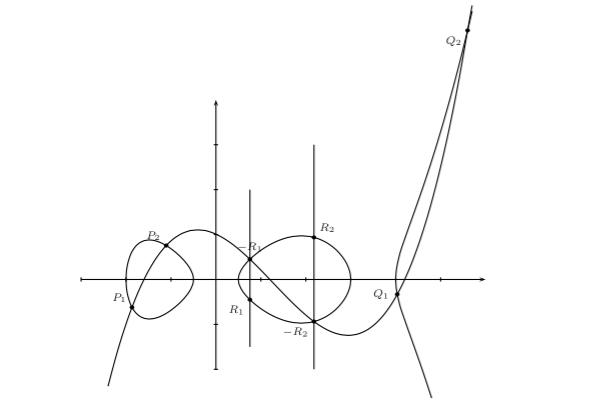
\includegraphics[width=11cm, height=7cm]{helliptic}
\end{center}

In an analogous way to elliptic curves, scalar multiplication of elements of $J$ may be computed using exponentiation by squaring. 

\subsection{Counting Points}

Just like in the case of elliptic curves, it is essential to determine the number of elements in $J$ over $\mathbb{F}_p$. We may use the generalized Hasse-Weil bound for a curve of genus $\mathfrak{g}$ to estimate the number of points in $J(\mathbb{F}_p)$. That is, 
$$
\sqrt{p} - 1)^{2\mathfrak{g}} + 1 \leq \# J(\mathbb{F}_p) \leq  \sqrt{p} - 1)^{2\mathfrak{g}} - 1
$$
An algorithm very analogous to Schoof's algorithm which works well for hyperelliptic curves of genus $\mathfrak{g} = 2$. Let $\phi$ be the Frobeneous endomorphism, then for genus $2$ curves, we get a similar eqaution of enddmorphism 
\begin{equation} \label{hypechar}
	\phi^4 + s_1  \phi^3 + s_2 \phi^2 - s_1q \phi + q^2 \equiv \OV 
\end{equation}
In the reverse direction, knowledge of  $\# J(\mathbb{F}_p)$ almost determines \eqref{hypechar} exactly. For example when the genus is $2$, $\# J(\mathbb{F}_p) - p^2 - 1 = s_2 -s_1(q+1)$. So the idea of the algorithm is to compute \eqref{hypechar} modulo small primes $l$ working in $J[l]$. Then Once this has been done, \eqref{hypechar} can be recovered using the Chinese remainder theorem in the exact same way as in Schoof's algorithm. A detailed implementation of this algorithm has been created in python but not included as pseudocode due to length. \\

The real advantage here is that the number of points in $J(\mathbb{F}_p)$ can be almost $g$ times greater than the number of points on a well suited elliptic curve $E(\mathbb{F}_p)$. Even when $g = 2$ this is a significant advantage. The bottleneck to using hyperelliptic curves is the group operation. It's arithmetic is combersome compared with that of elliptic curves and this is only exacerbated when the size of $p$ is large.  





